%\chapter{Problem and Its Background}
\chapter{INTRODUCTION}

\section{Background of the Study}

% AI Game engine prog p 415
Genetic algorithms are one of the many types of artificial intelligence
techniques that exist today. If implemented well, genetic algorithms can
evolve a computer controlled agent to perform adequately according to some
set criteria defined in a fitness function. However, a significant amount of 
time is required for the algorithm to evolve a population of individual solutions 
into an acceptable solution\cite{Schwab04}. The time it takes can range from
a few hours to a number of weeks, depending on the complexity of the game where
the agent must perform. This limitation makes them difficult or impractical to
use in the process of game development\cite{Schwab04}.

% refer to the bottom part of p 415 and top part of p 417 in AI game engine prog
The primary reasons genetic algorithms take up a lot of time are the number of 
possible solutions that must be tested given a specific generation, the time it 
takes to evaluate each of these possible solutions, and the number of generations 
that may be needed before arriving at a single or a number of acceptable solutions\cite{Schwab04}. 
One way to tackle the issue is by using faster processors in order to reduce the
overall computation time of the Genetic Algorithm. A better solution though would
be to process all the individuals in a single generation in parallel through the
use of threads. A computer processor is capable of a variety of things, but it can only process
one instruction at a time. This is where Graphics Processing Units, or GPUs, come in.
GPUs have been designed to execute a single set of instructions over numerous elements
of data, a technique known as ``Single-Instruction, Multiple-Thread\cite{pdf:NVCudaPrgGuide}.''
Not only do they have multiple processing units, each processing unit is also
capable of running several identical instructions simultaneously, making GPUs ideal
for highly parallel algorithms\cite{pdf:NVCudaPrgGuide}. It is our goal therefore to
show that GPUs can be used to evolve an optimized solution for the behavior of computer
controlled agents in a computer game at a rate that is much faster than those that are optimized
through the use of a CPU.

\begin{figure}
	\centering
		\graphicspath{{images/}}
		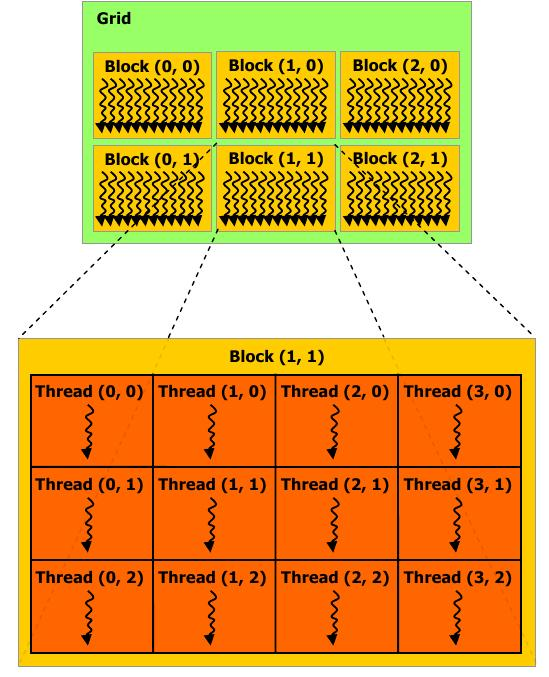
\includegraphics[width=450 pt]{gpu.jpg}
	\caption{Concurrent threads in a GPU organized in thread blocks, all of which
are running in parallel}
	\cite{pdf:NVCudaPrgGuide}
	\label{fig:gpu_diagram}
\end{figure}

\section{Research Objectives}

The objective of this study is to show that the GPU can be used to reduce the time
it takes to optimize game AI and thus make them more practical for use during the
development process of computer games. This research aims to illustrate the
performance gains of using a GPU to optimize the AI with the use of Genetic Algorithms.


\section{Research Question}

In order to complete the research objective of illustrating the benefits of using
a GPU for optimizing game AI, we will need to answer the following questions:

\begin{enumerate}
 \item Which parts of the AI can we optimize through the use of genetic algorithms?

 \item How do we structure the game such that most of the code may be shared between
the actual game and the offline tool that utilizes the GPU?

 \item How much faster can the GPU based application generate an optimized ``gene''
as compared to a CPU based implementation?
\end{enumerate}

\section{Scope and Limitations}

The focus of the study is in determining the performance gains that can be attained from
running the genetic algorithm on the GPU. As such, the main variable in this study is the
average running time of the application in generating an optimal solution. Although there
are many other factors that would determine whether this approach to optimizing game AI
is practical, they will have to be the subject of further research due to the limited time
available for this study.


\section{Significance}

Genetic algorithms have applications over a wide variety of fields.
Inspired by evolutionary biology, it can find the optimal solution
for a given problem. For example, artificial neural networks (ANN),
are used in the manufacturing industry to identify the best parameters
for constructing a model. Genetic algorithm based ANNs are found to be
the best due to its time-saving potential\cite{Venkatesan08}. Another
application can be found in the field of traffic control. They used
genetic algorithm to design an optimal toll ring scheme to reduce traffic
congestion\cite{Sumalee08}. Other applications can be found in the field
of Game AI. For example, we can make more sophisticated AI using genetic
algorithms. These AIs will be smarter in the sense that they can ``learn''.
This aspect of AI can make it more challenging, a very valuable element
in a computer game. With the age of graphics reaching its peak, the need
for better AI is starting to become an ingredient for a succesful
commercial game\cite{Yue06}. Because of the inherent ability of genetic
algorithms in learning, AIs can be made more robust. They could display
behaviors that were not seen in the previous playthrough. Thus, this
could make more challenging AIs after each playthrough. An application
of this can be seen in an experiment to create an intelligent player
for a game titled ``Megaman 2\cite{website:Kuliniewicz09}.'' Here the
computer controlled player played by trying different sets of inputs
to defeat a particular boss named ``Air Man.'' With each generation,
the computer player performed better than its previous playthrough
until it had reached the point wherein its fitness score would no longer
increase. 


%Other applications of genetic algorithm can be found in companies like First Quadrant Corp.
%It is an investment management firm that used genetic algorithms to model yield on 
%investment funds\cite{website:Davis}. Through this method, they are have a
%``significant improvement'' of over USD 128 Billion under investment\cite{website:Davis}.
%Furthermore, in the field of Telecommunications, Cox Associates is using genetic
%algorithms for their cellular clients\cite{website:Davis}. As a result, they are
%saving millions of dollars. Another application can be found in the field of traffic
%control, specifically in traffic lights and pedestrian crossing control\cite{Turky09}.


Various studies have already been done in the fields of genetic algorithm with
some of the applications being used commercially. However, it would seem that there
has yet to be any study done in improving genetic algorithms using the GPU for optimizing
game AI. It has been proven that genetic algorithms are limited and impractical without
the processing power of the GPU\cite{Banzhaf09}. Without this limitation however, GAs
could be used to optimize game AI in place of manually hand tuning them. Not only does
this have the potential to reduce the time it takes to fine-tune the game AI, it will
also allow the game developer/designer to work on other tasks while the computer
does the fine-tuning.